% REPORT FOR PROJECT2 SF2565

\documentclass[a4paper,10pt]{article}

%%Packages	%%%	%%%	%%%	%%%	%%%	%%%	%%%
\usepackage{amsmath,framed}
\usepackage[latin1]{inputenc} 	
\usepackage{listings}
\usepackage{xcolor}
\usepackage{graphicx}
\usepackage{placeins}
\usepackage{tikz}

%%Settings	%%%	%%%	%%%	%%%	%%%	%%%	%%%
\renewcommand{\d}{\text{d}}
\newcommand{\e}{\text{e}}
\newcommand{\ve}{\mathbf}
\newcommand\numb{\addtocounter{equation}{1}\tag{\theequation}}

\setlength\fboxsep{1.2mm}
\setlength\fboxrule{0.5mm}

\lstset { %
  language=C++,
  backgroundcolor=\color{black!3},	% set backgroundcolor
  basicstyle=\footnotesize,		% basic font setting
}

%%Margins	%%%	%%%	%%%	%%%	%%%	%%%	%%%
\usepackage{geometry}
\geometry{
  a4paper,
  left=35mm,
  right=35mm,
  top=35mm,
  bottom=35mm,
}

%%Header & Footer	%%%	%%%	%%%	%%%	%%%	%%%
\usepackage{fancyhdr}
\pagestyle{fancy}
\renewcommand{\headrulewidth}{1pt}
\rhead{Hanna Hultin, Mikael Perssson}
%8509080456 mitt persnr om vi vill ha det
\lhead{P2 SF565}

\title{Project 3, SF2565}
\author{Hanna Hultin, hhultin@kth.se, 931122-2468, TTMAM2 \\ Mikael Persson, mikaepe@kth.se, 850908-0456, TTMAM2}
\begin{document}
\maketitle

\subsection*{Short review}
Given a domain $D$ enclosed by four curves $\ve{x}_i (p_i), \enspace i = 1,2,3,4,$  
(where $p_i$ are any suitable parameters for the curves)
we want to generate a structured grid on the domain.
For this we define grid parameters $\xi_1 \in [0,1]$ and $\xi_2 \in [0,1]$.
The unit square $R = [0,1]\times[0,1]$ is discretized using 
\begin{align*}
  \xi_{1,i} &= i h_1,\quad i = 0,1,\dots,n, \\
  \xi_{2,j} &= j h_2,\quad j = 0,1,\dots,m.
\end{align*}
where $h_1 = 1/n$ and $h_2 = 1/m$. Define linear interpolation functions $\phi_1(x) = 1$ and
$\phi_2(x) = 1-x$.
Assuming bijective maps $\Phi_1 : [0,1] \mapsto \ve{x}_1(p_1)$ and similarly for the three other
boundaries, the grid may now be generated using the algebraic grid generation formula:
\begin{align*}
  \ve{x}_{ij} &= \phi_2(\xi_{1,i}) \Phi_4 (\xi_{2,j}) + \phi_1(\xi_{1,i}) \Phi_2(\xi_{2,j}) 
  &&\text{[left to right interpolation]}\\
  &\hspace{1mm}+ \phi_2(\xi_{2,j}) \Phi_1(\xi_{1,i}) + \phi_1(\xi_{2,j}) \Phi_3(\xi_{1,i})
  &&\text{[bottom to top interpolation]} \\
  &\hspace{1mm}- \phi_2(\xi_{1,i}) \phi_2(\xi_{2,j}) \Phi_1(0) - 
  \phi_1(\xi_{1,i}) \phi_2(\xi_{2,j}) \Phi_1(1) 
  &&\text{[corrections, corners]}\\
  &\hspace{1mm}- \phi_2(\xi_{1,i}) \phi_1(\xi_{2,j}) \Phi_3(0) -
  \phi_1(\xi_{1,i}) \phi_1(\xi_{2,j}) \Phi_3(1)
  .
\end{align*}

\begin{figure}[!ht]
  \centering
  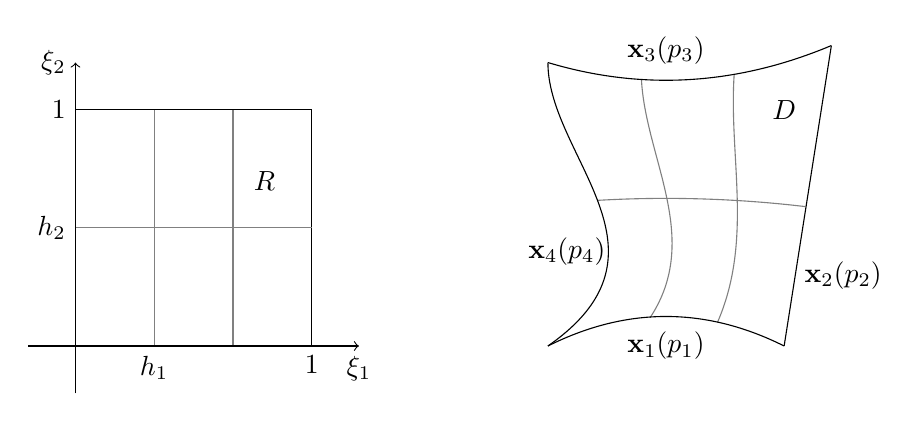
\begin{tikzpicture}[scale = 3.0]

    \draw (0,0) -- (1,0) -- (1,1) -- (0,1) -- cycle;

    \draw[color = gray] (0,.5) -- (1,.5);
    \draw[color = gray] (.333,0) -- (.333,1);
    \draw[color = gray] (.667,0) -- (.667,1);

    \node[anchor = north] at (.333,0) {$h_1$};
    \node[anchor = east] at (0,.5) {$h_2$};

    \node[anchor = north] at (1,0) {1};
    \node[anchor = east] at (0,1) {1};

    \draw[->] (-.2,0) -- (1.2,0) node [anchor = north] {$\xi_1$};
    \draw[->] (0,-.2) -- (0,1.2) node [anchor = east] {$\xi_2$};



    \node at (.8,.7) {$R$};


    \draw[color = gray, smooth, samples = 50, domain=2.21:3.09] plot(\x,
    -0.5*0.5*\x*\x +0.5*0.3*\x*\x + 0.5*2.5*\x - 0.5*1.5*\x -0.5*3 + 0.5*3);

    
    \draw[color = gray, smooth, samples = 50, domain = 0.1:1.15] 
    plot(0.333*\x*\x*\x-0.333*2.4*\x*\x + 0.333*1.44*\x + 0.333*2 + 0.667*0.15723*\x+0.667*3,\x); 
    
    \draw[color = gray, smooth, samples = 50, domain = 0.12:1.13] 
    plot(0.667*\x*\x*\x-0.667*2.4*\x*\x + 0.667*1.44*\x + 0.667*2 + 0.333*0.15723*\x+0.333*3,\x); 

    % Horizontal curves
    \draw[smooth, samples = 50, domain=2:3] plot(\x,-0.5*\x*\x + 2.5*\x -3);
    \draw[smooth, samples = 50, domain=2:3.2] plot(\x,0.3*\x*\x - 1.5*\x +3);


    % Vertical curves
    \draw[smooth, samples = 50, domain = 0:1.2] plot(\x*\x*\x-2.4*\x*\x + 1.44*\x + 2, \x); 
    \draw[smooth, samples = 50, domain = 0:1.272] plot(0.15723*\x+3,\x);
 

    \node at (2.5,0) {$\ve{x}_1 (p_1)$};
    \node at (3.25,.3) {$\ve{x}_2 (p_2)$};
    \node at (2.5,1.25) {$\ve{x}_3 (p_3)$};
    \node at (2.08,0.4) {$\ve{x}_4 (p_4)$};

    \node at (3,1) {$D$};



  \end{tikzpicture}


  \begin{minipage}[t]{100mm}
    \caption{
      The domain $D$ is enclosed by four curves parametrized by the parameter $p$.
      The grid is generated using maps from the boundary curves of 
      $[0,1]\times [0,1]$ to the boundary curves of the domain $D$.
    }
    
    \label{FIG_jjj}
  \end{minipage}
\end{figure}

\FloatBarrier

\subsection*{Task 1: The Curvebase class}
In this project we use an abstract class \texttt{Curvebase} to represent curves. The class is written so that it should be easy to derive different classes from \texttt{Curvebase} to represent a wide range of different curves.

We have private virtual functions for determining the value of $x$ and $y$ as well as the derivatives with respect to $x$ and $y$ for the curve given the user parameter $p$. $p$ is supposed to take values between $a$ and $b$ which are private members of the class. We also have a private member variable called \texttt{length} which is supposed to be the arc length of the curve. 

We have public member functions for determining $x$ and $y$ given the parameter $s$ which is a scaled parameter that goes from $0$ to $1$. To determine the corresponding $x$ and $y$ we use a private member function called \texttt{newtonsolve} which uses Newton's method. To compute the integral of the arc length between two values $a$ and $b$ \texttt{newtonsolve} calls the private function \texttt{integrate}. This function uses the private member functions \texttt{iSimpson} and \texttt{i2Simpson} to compute the integral according to Project 1. 

\subsection*{Task 2: The derived classes}
From the abstract class \texttt{Curvebase} we derived the classes \texttt{xLine}, \texttt{yLine} and \texttt{fxcurve} to be able to create the boundary curves for the desired grid.

\texttt{xLine} is a class that represents curves which has a constant $y$-value. Here we set $a$ to be the initial value of $x$, $b$ the final value of $x$ and length is just set to $b-a$ since we have a straight line. We also have a private variable for the constant $y$-value called $yConst$.

We use $x$ as the used parameter so the private functions for determining the values of $x$ and $y$ and the derivatives just becomes: $x(p)=p$, $y(p)=yConst$, $dx(p)=1$ and $dy(p)=0$.

We also use that we can overwrite the functions for determining $x$ and $y$ given the parameter $s$ since in this special case these values can be computed easily. So we use that $x(s) = a+s*length$ and $y(s) = yConst$. We also use that the arc length integral between $x_1$ and $x_2$ is just $x_2-x_1$.

\texttt{yLine} is a class that represents curves which has a constant $x$-value. For \texttt{yLine} everything looks the same as for \texttt{xLine} but with $x$ and $y$ interchanged everywhere.

Lastly we have the class \texttt{fxcurve}. This is a specific class used to to represent the given lower boundary curve. Here we use $x$ as the user parameter $p$ and then we implemented that $x(p) = p$, $y(p) = f(p)$, $dx(p) = 1$ and $dy(p) = f'(p)$ where $f(\cdot)$ is given in the project description and expression for the derivative was computed analytically.  
 

\subsection*{Task 3: The Domain class}
In this task we designed the class Domain which is a general class for modelling 4-sided domains and structured grids on them. This class takes references to four objects of type \texttt{Curvebase} as arguments to the constructor. The curves represented by these \texttt{Curvebase} objects are then the four sides of the \texttt{Domain}. 


The class \texttt{Domain} has a public member function called \texttt{grid\_generation} which generates a grid according to the algebraic grid generation formula.

\subsection*{Task 4: Writing the grid to a file and plotting it in Matlab}
To be able to write the generated grid to a file we added the public function \texttt{writeFile} to our class \texttt{Domain}. This function opens a binary file and writes first all the $x$-values for the grid points and then the $y$-values for all the grid points before closing the file. 

We then opened the binary file in Matlab and plotted the grid points. 

\begin{figure}[!ht]
  \centering
  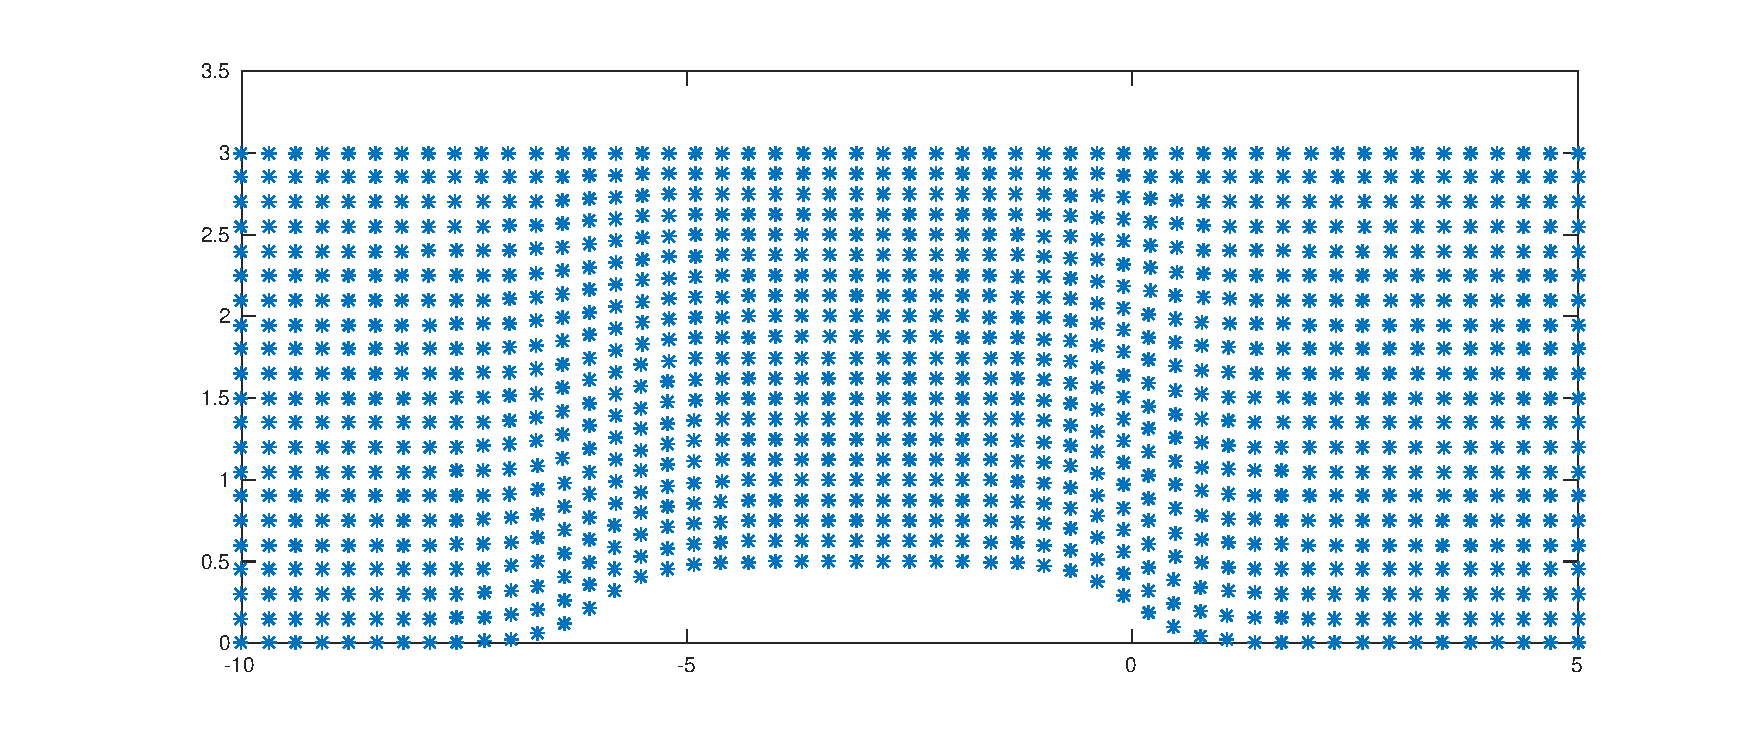
\includegraphics[width = 13cm, height = 8cm]{50x20}
  \begin{minipage}[t]{100mm}
    \caption{
      The generated grid using $n = 50$ and $m = 20$.
    }\label{FIG_jjj}
  \end{minipage}
\end{figure}


\newpage
\subsection*{Code}
\subsubsection*{Main}
\lstinputlisting[language=C++,basicstyle=\scriptsize]{../main1.cpp}
\subsubsection*{Task 1: The Curvebase Class}
\lstinputlisting[language=C++,basicstyle=\scriptsize]{../curvebase.hpp}
\lstinputlisting[language=C++,basicstyle=\scriptsize]{../curvebase.cpp}
\subsubsection*{Task 2: The derived classes}
\lstinputlisting[language=C++,basicstyle=\scriptsize]{../xline.hpp}
\lstinputlisting[language=C++,basicstyle=\scriptsize]{../xline.cpp}
\lstinputlisting[language=C++,basicstyle=\scriptsize]{../yline.hpp}
\lstinputlisting[language=C++,basicstyle=\scriptsize]{../yline.cpp}
\lstinputlisting[language=C++,basicstyle=\scriptsize]{../fxcurve.hpp}
\lstinputlisting[language=C++,basicstyle=\scriptsize]{../fxcurve.cpp}
\subsubsection*{Task 3 and 4: The Domain Class}
\lstinputlisting[language=C++,basicstyle=\scriptsize]{../domain.hpp}
\lstinputlisting[language=C++,basicstyle=\scriptsize]{../domain.cpp}



\end{document}





